The breast cancer dataset was the second mandatory dataset. We got a score of 97.647\% on kaggle.

\subsection{Characteristics}

\begin{itemize}
\item No missing values
\item binary target class (B and M)
\item Only rational features
\item 30 attributes (disregarding id)
\item 285 samples
\end{itemize}


\subsection{Characteristics of Target Value}

There are two target classes, B and M (B=bengin, M=malignant). While 96 of the samples are of type M, 189 are of type B. A tumor is a cluster of abnormal cells, if it is a benign tumors do not contain cancerous cells, while malignant tumors do hold cancerous cells. Therefore it is more important to correctly classifiy a sample if it is a malignant tumor than correctly classifing a bengin tumor.


\image{breast/plots/countplot.png}{Histogram of the target values}{\label{fig:breast-target}}

% \begin{figure}[H]
%   \begin{center}
%     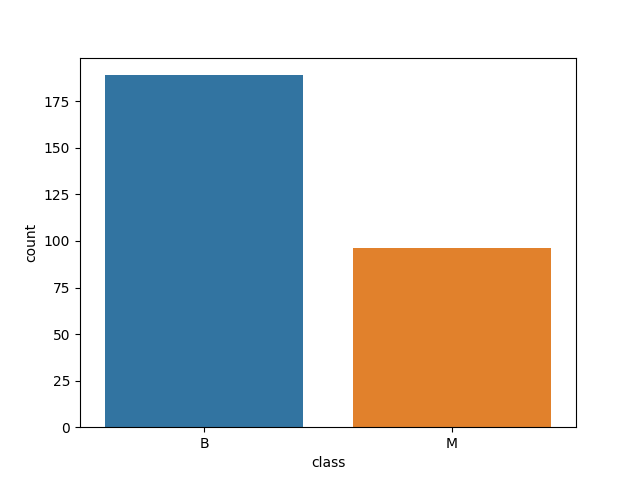
\includegraphics[width=0.8\linewidth]{breast/plots/countplot.png}
%     \caption{Histogram of the target values}
%     \label{fig:breast-target}
%   \end{center}
% \end{figure}

\subsection{Feature Selection}
First different plots to visualize the data were made. An example can be seen in Figure \ref{fig:breast-violin}. In the example it can be seen that the fractalDimensionMean (the feature on the right) is bad for classification while the radiusMean could be useful.

\image{breast/plots/violinplot.png}{Violine plot of the first 10 features that were scaled by minmax}{\label{fig:breast-violin}}

% \begin{figure}[H]
%   \begin{center}
%     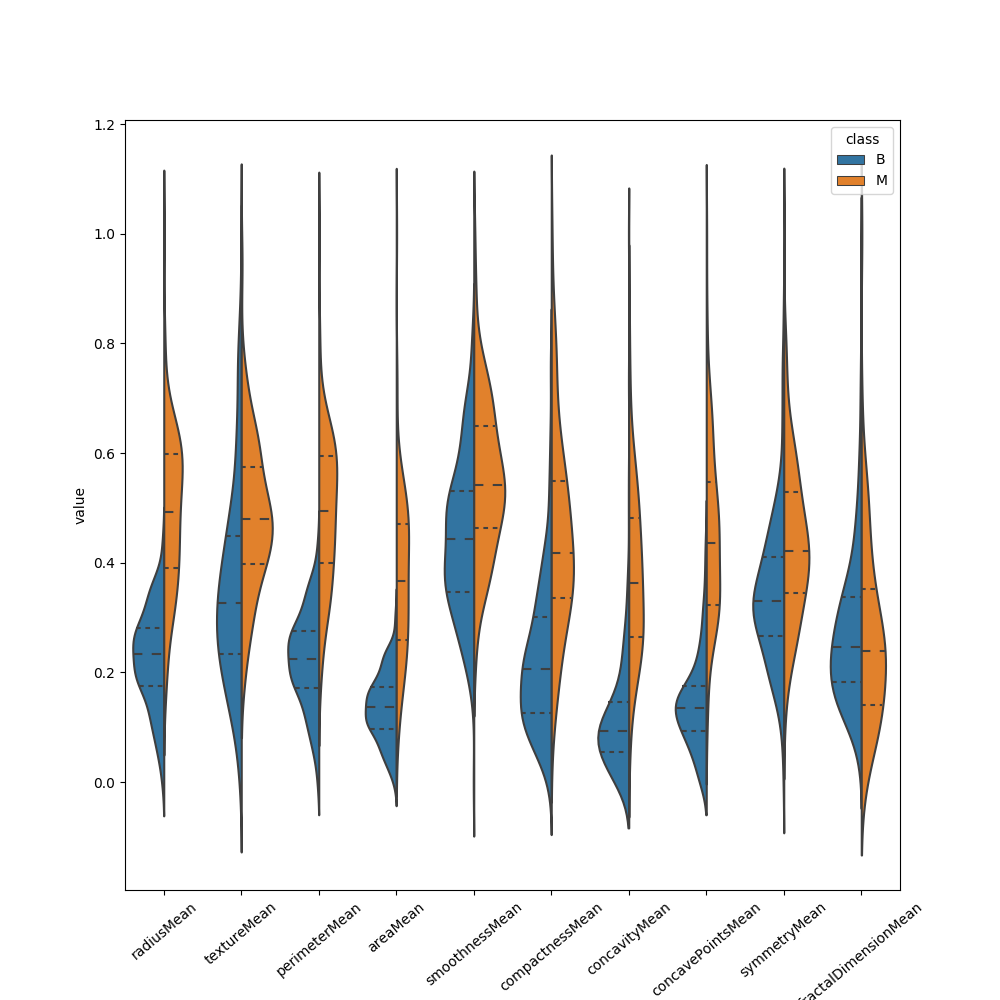
\includegraphics[width=0.8\linewidth]{breast/plots/violinplot.png}
%     \caption{Histogram of the target values}
%     \label{fig:breast-violin}
%   \end{center}
% \end{figure}

Also recursive feature selection was tried, as seen in Figure \ref{fig:breast-feature-selection} 15 to 30 features work best.

\image{breast/plots/rf_feature_selection.png}{Recursive Feature selection}{\label{fig:breast-feature-selection}}

\subsection{K Nearest Neighbors Classifier}

Similarily to the iris dataset \textit{GridSearchCV} was used to test different Ks and metrics. As seen in Figure \ref{fig:breast-knn-metrics} euclidean works best. 

\image{breast/plots/knn_p_comparision.png}{Comparison of metrics}
% \begin{figure}[H]
%   \begin{center}
%     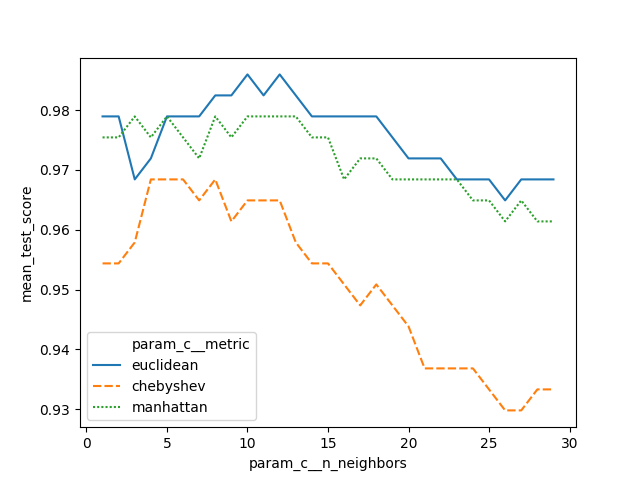
\includegraphics[width=0.8\linewidth]{breast/plots/knn_p_comparision.png}
%     \caption{Histogram of the target values}
%     \label{fig:breast-knn-metrics}
%   \end{center}
% \end{figure}

As seen in Figure \ref{fig:breast-knn-comparison} preprocessing is actually worse than without preprocessing.

\begin{figure}[H]
  \begin{center}
    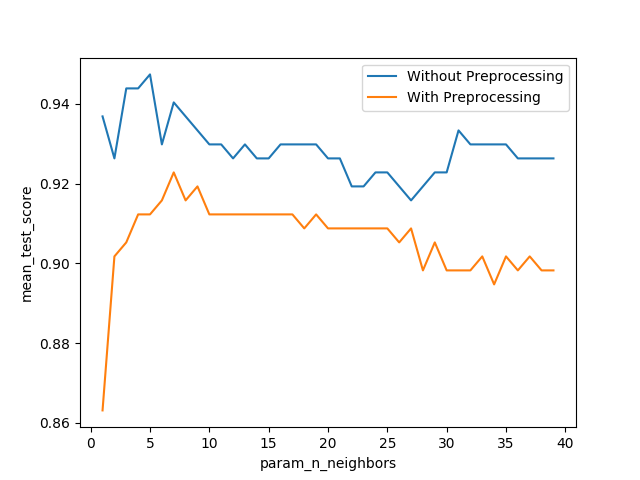
\includegraphics[width=0.8\linewidth]{breast/plots/knn_feature_comparision.png}
    \caption{Histogram of the target values}
    \label{fig:breast-knn-comparison}
  \end{center}
\end{figure}

\subsection{Random Forest Classifier}

As shown in Figure \ref{fig:breast-rf-comparison}

\begin{figure}[H]
  \begin{center}
    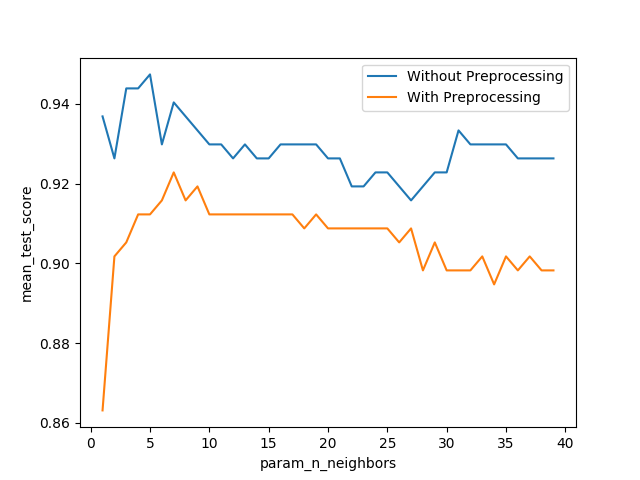
\includegraphics[width=0.8\linewidth]{breast/plots/knn_feature_comparision.png}
    \caption{Comparison of Random Forest with and without Preprocessing}
    \label{fig:breast-rf-comparison}
  \end{center}
\end{figure}

\subsection{Multi-Layer Perceptron Classifier}

\image{breast/plots/mlp_p_comparision.png}{comparison of layer sizes and activation functions}{\label{fig:breast-mlp-comparison}}

\subsection{Conclusion}

\begin{table}[H]
\begin{center}
\begin{tabular}{|l|l|l|}
\hline
                       & Preprocessing & No-Preprocessing \\ \hline
KNeighborsClassifier   & 0.9862        & 0.9474           \\ \hline
RandomForestClassifier & 0.9789        & 0.9789           \\ \hline
MLPClassifier          & 0.9824        & 0.9614           \\ \hline
\end{tabular}
\caption{Comparison of accuracy of different techniques with- and without preprocessing}
\end{center}
\end{table}

\begin{table}[H]
\begin{center}
\begin{tabular}{|l|l|l|}
\hline
                       & Holdout & Cross Validation \\ \hline
KNeighborsClassifier   & 0.9824  & 0.9862           \\ \hline
RandomForestClassifier & 0.9824  & 0.9789           \\ \hline
MLPClassifier          & 0.9824  & 0.9858           \\ \hline
\end{tabular}
\caption{Comparison of accuracy of holdout versus cross-validation}
\end{center}
\end{table}

\begin{table}[H]
\begin{center}
\begin{tabular}{|l|l|l|l|l|l|}
\hline
                       & Accuracy & Precision & Recall & F1     & Runtime (sec) \\ \hline
KNeighborsClassifier   & 0.9862   & 0.9902    & 0.9800 & 0.9841 & 0.0016        \\ \hline
RandomForestClassifier & 0.0756   & 0.9752    & 0.9715 & 0.9726 & 0.0677        \\ \hline
MLPClassifier          & 0.9858   & 0.9902    & 0.9783 & 0.9831 & 0.8999        \\ \hline
\end{tabular}
\caption{Comparison of different performance metrics and runtimes}
\end{center}
\end{table}

